%+++++++++++++++++++++++++++++++++++++++++++++++++++++++++++++++
% SUMMARY    : Dimensionality, Distance, and KNN
%            : University of Southern Maine 
%            : @james.quinlan
%            : Sarah Lawrence  - Lecture 3 --> updated by Mohamed Noor
%+++++++++++++++++++++++++++++++++++++++++++++++++++++++++++++++

% Define colors for consistency in figures
\definecolor{pointcolor}{RGB}{0,0,0}
\definecolor{highlightcolor}{RGB}{128,0,128}
\definecolor{specialpoint}{RGB}{255,0,0}
\definecolor{positiveclass}{RGB}{0,128,0}
\definecolor{negativeclass}{RGB}{255,0,0}

\section*{Objectives}
\begin{outline}
  \1 Understand the concept of dimensionality and its implications in machine learning
  \1 Learn different distance metrics and their applications
  \1 Master the K-Nearest Neighbors algorithm for classification and regression
\end{outline}

\rule[0.0051in]{\textwidth}{0.00025in}
% ----------------------------------------------------------------

\section{Review of Vector Spaces}
\subsection{Vector Notation}
\[
\vec{x} \in {\mathbb{R}}^p
\]

\begin{outline}
    \1 $\vec{x}$ represents a vector (a data point with multiple attributes) 
    \1 $\in$ represents an element belonging to a particular set 
    \1 $\mathbb{R}$ represents the set of all real numbers 
    \1 $p$ represents the dimension of the vector space (number of features) 
    \1 \textbf{Meaning}: $\vec{x}$ is a vector with all elements being real numbers in $p$-dimensional space
    \1 \textbf{Terminology}: $p$ is also known as the Feature Space dimension, Number of Factors, or Number of Variables
\end{outline}

In practice, we typically represent a vector as a column vector:
$\vec{x} = \begin{bmatrix}
x_1 \\
x_2 \\
\vdots \\
x_p
\end{bmatrix}$ 
where each $x_i$ represents a specific feature or attribute of our data point.

\subsection{Distance Fundamentals}
\[
    d(x,y)
\]
\textbf{Distance metric}: Measures the dissimilarity between two points $x$ and $y$. A proper distance metric must satisfy several properties:
\begin{outline}
    \1 Non-negativity: $d(x,y) \geq 0$
    \1 Identity of indiscernibles: $d(x,y) = 0$ if and only if $x = y$
    \1 Symmetry: $d(x,y) = d(y,x)$
    \1 Triangle inequality: $d(x,z) \leq d(x,y) + d(y,z)$
\end{outline}

The most common distance metric is Euclidean distance:
\[
    d(x,y) = ||x-y|| = \sqrt{\sum_{i=1}^{p} (x_i - y_i)^2}
\]

\subsection{Dimensionality Challenges}
When the number of dimensions is large, we encounter:
\[
    p \gg 1
\]
\textbf{Meaning}: The vector $x$ has a high number of dimensions.

\textbf{Challenges}: High dimensionality introduces several problems:
\begin{outline}
    \1 Data sparsity: Points become increasingly distant from each other
    \1 Computational complexity: More dimensions mean more calculations
    \1 Overfitting: Models can fit noise in high-dimensional spaces
    \1 The ``Curse of Dimensionality": A collection of phenomena that make analysis more difficult as dimensions increase
\end{outline}

\section{Dimensionality in Detail}
\subsection{Understanding the Space}

Two-dimensional vector space with uniformly distributed points:

\begin{center}
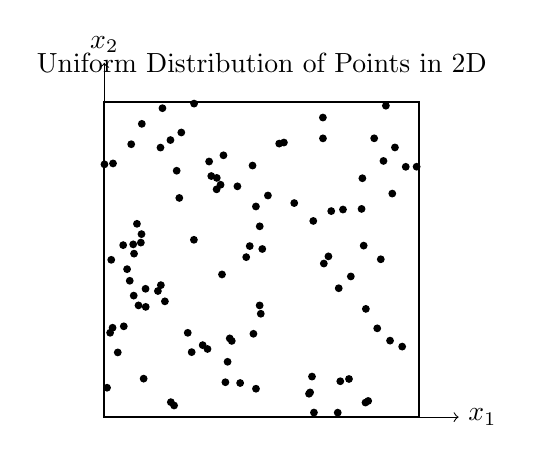
\begin{tikzpicture}
  % Draw the box with axis labels
  \draw[thick] (0,0) rectangle (4,4);
  \draw[->] (0,0) -- (4.5,0) node[right] {$x_1$};
  \draw[->] (0,0) -- (0,4.5) node[above] {$x_2$};

  % Generate random dots inside the box
  \foreach \i in {1,...,100} {
    \node[circle, fill=pointcolor, inner sep=1pt] at ({4*rnd}, {4*rnd}) {};
  }

  % Add title
  \node[align=center] at (2,4.5) {Uniform Distribution of Points in 2D};
\end{tikzpicture}
\end{center}

\subsection{The Curse of Dimensionality}
\textbf{Definition}: The "Curse of Dimensionality" refers to various phenomena when analyzing data in high-dimensional spaces that do not occur in low-dimensional settings.

\textbf{Key insight}: In a feature space with $p$ dimensions, $[0,1]^p$, filled with randomly distributed points, as $p$ increases:
\begin{outline}
    \1 The average distance between points increases
    \1 The average distance from any point to the nearest edge decreases
    \1 Volume concentrates near the edges and corners
\end{outline}

This effect is illustrated below, where points tend to cluster near the edges in higher dimensions:

\begin{center}
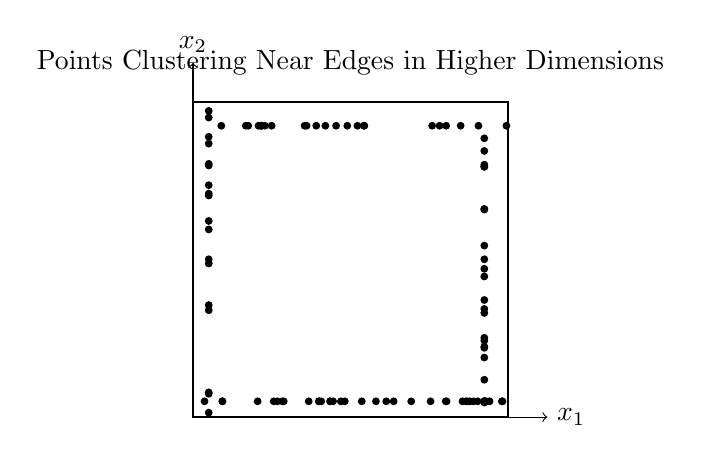
\begin{tikzpicture}
  % Draw the 4x4 box
  \draw[thick] (0,0) rectangle (4,4); 
  \draw[->] (0,0) -- (4.5,0) node[right] {$x_1$};
  \draw[->] (0,0) -- (0,4.5) node[above] {$x_2$};

  % Generate random dots near all four edges
  \foreach \i in {1,...,100} {
    \pgfmathsetmacro{\edgeSelector}{int(rnd*4)} 
    \pgfmathsetmacro{\pos}{rnd*4} 

    \ifnum \edgeSelector=0
      \node[circle, fill=pointcolor, inner sep=1pt] at (\pos, 0.2) {}; % Bottom edge
    \else
      \ifnum \edgeSelector=1
        \node[circle, fill=pointcolor, inner sep=1pt] at (\pos, 3.7) {}; % Top edge
      \else
        \ifnum \edgeSelector=2
          \node[circle, fill=pointcolor, inner sep=1pt] at (0.2, \pos) {}; % Left edge
        \else
          \node[circle, fill=pointcolor, inner sep=1pt] at (3.7, \pos) {}; % Right edge
        \fi
      \fi
    \fi
  }

  % Add title
  \node[align=center] at (2,4.5) {Points Clustering Near Edges in Higher Dimensions};
\end{tikzpicture}
\end{center}

\subsection{Dimensionality Reduction}
\textbf{Definition}: Dimensionality reduction techniques aim to reduce the number of features while preserving as much relevant information as possible.

Visual representation of dimensionality reduction from 3D to 2D:

\begin{center}
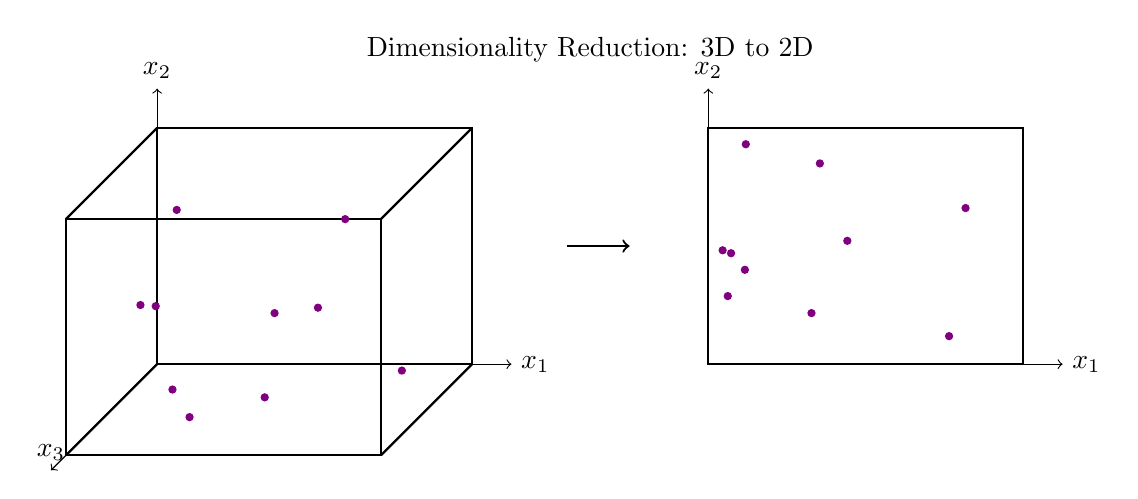
\begin{tikzpicture}
% Coordinates for 3D cube
\coordinate (A) at (0,0,0);
\coordinate (B) at (4,0,0);
\coordinate (C) at (4,3,0);
\coordinate (D) at (0,3,0);
\coordinate (E) at (0,0,3);
\coordinate (F) at (4,0,3);
\coordinate (G) at (4,3,3);
\coordinate (H) at (0,3,3);

% Box lines
\draw[thick] (A) -- (B) -- (C) -- (D) -- cycle; % Bottom
\draw[thick] (E) -- (F) -- (G) -- (H) -- cycle; % Top
\draw[thick] (A) -- (E);
\draw[thick] (B) -- (F);
\draw[thick] (C) -- (G);
\draw[thick] (D) -- (H);

% Add axis labels to 3D cube
\draw[->] (0,0,0) -- (4.5,0,0) node[right] {$x_1$};
\draw[->] (0,0,0) -- (0,3.5,0) node[above] {$x_2$};
\draw[->] (0,0,0) -- (0,0,3.5) node[above] {$x_3$};

% Add random points in 3D
\foreach \i in {1,...,10} {
    \pgfmathsetmacro{\x}{rnd*4} 
    \pgfmathsetmacro{\y}{rnd*3}
    \pgfmathsetmacro{\z}{rnd*3}
    \fill[highlightcolor] (\x,\y,\z) circle (1.5pt);
}

% Add arrow and 2D projection
\draw[->, thick] (5.2, 1.5) -- (6, 1.5);

\begin{scope}[shift={(7,0)}]
    % 2D box with axis labels
    \draw[thick] (0,0) rectangle (4,3);
    \draw[->] (0,0) -- (4.5,0) node[right] {$x_1$};
    \draw[->] (0,0) -- (0,3.5) node[above] {$x_2$};

    % Add projected points in 2D
    \foreach \i in {1,...,10} {
        \pgfmathsetmacro{\x}{rnd*4} 
        \pgfmathsetmacro{\y}{rnd*3}
        \fill[highlightcolor] (\x,\y) circle (1.5pt);
    }
\end{scope}

% Add title
\node[align=center] at (5.5,4) {Dimensionality Reduction: 3D to 2D};

\end{tikzpicture}
\end{center}

\subsection{The Box Size Problem}
An essential question in high-dimensional spaces: What is the box size $\ell$ that always contains exactly $k$ points?

Key parameters:
\begin{outline}
    \1 $k$ = fixed number $<$ $n$ (number of points we want inside the box)
    \1 $n$ = total number of samples (total points in the space)
    \1 $p$ = number of dimensions
    \1 Terminology: If $p$ is $\geq 4$ we call it a \textbf{hyper-cube}
\end{outline}

\textbf{Example 1}: $k = 1$, $p = 1$, $n = 7$ points distributed on a line

\begin{center}
    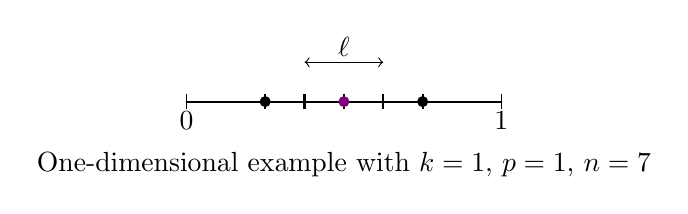
\begin{tikzpicture}
        % Draw the line segment
        \draw[thick] (0,0) -- (4,0);

        % Add labels at 0 and 1
        \node[below] at (0,0) {0};
        \node[below] at (4,0) {1};

        % Draw small ticks and points
        \draw (0,0.1) -- (0,-0.1);
        \draw[thick] (1,0.1) -- (1,-0.1);
        \fill[pointcolor] (1,0) circle (2pt) node[above] {};

        \draw[thick] (1.5,0.1) -- (1.5,-0.1);

        \draw[thick] (2,0.1) -- (2,-0.1);
        \fill[highlightcolor] (2,0) circle (2pt) node[above] {};

        \draw[thick] (2.5,0.1) -- (2.5,-0.1);

        \draw[thick] (3,0.1) -- (3,-0.1);
        \fill[pointcolor] (3,0) circle (2pt) node[above] {};

        \draw (4,0.1) -- (4,-0.1);

        % Add the box length
        \draw[<->] (1.5,0.5) -- (2.5,0.5);
        \node at (2, 0.7) {$\ell$};

        % Title
        \node[align=center] at (2,-0.8) {One-dimensional example with $k=1$, $p=1$, $n=7$};
    \end{tikzpicture}
\end{center}

\textbf{Example 2}: $k = 3$, $p = 2$, $n = 100$ points in a plane

\begin{center}
    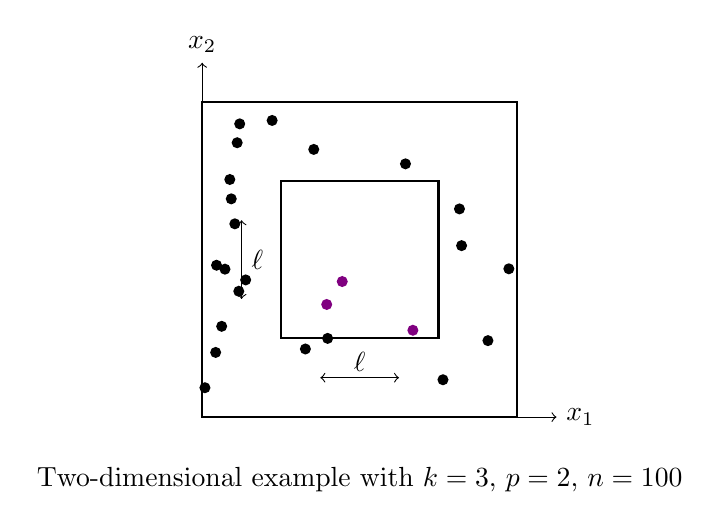
\begin{tikzpicture}
      % Draw outer and inner boxes
      \draw[thick] (0,0) rectangle (4,4);
      \draw[thick] (1,1) rectangle (3,3);

      % Add axis labels
      \draw[->] (0,0) -- (4.5,0) node[right] {$x_1$};
      \draw[->] (0,0) -- (0,4.5) node[above] {$x_2$};

      % Generate 3 fixed dots inside the inner square
      \foreach \i in {1,2,3} {
        \pgfmathsetmacro{\x}{1 + rnd*2} % Random x between 1 and 3
        \pgfmathsetmacro{\y}{1 + rnd*2} % Random y between 1 and 3
        \fill[highlightcolor] (\x,\y) circle (2pt);
      }

      % Generate random dots outside the inner square but within the big box
      \foreach \i in {1,...,25} {
        \pgfmathsetmacro{\x}{rnd*4} % Random x within the outer box
        \pgfmathsetmacro{\y}{rnd*4} % Random y within the outer box
        % Ensure points are outside the inner box
        \ifdim \x pt < 1 pt \fill[pointcolor] (\x,\y) circle (2pt);
        \else \ifdim \x pt > 3 pt \fill[pointcolor] (\x,\y) circle (2pt);
        \else \ifdim \y pt < 1 pt \fill[pointcolor] (\x,\y) circle (2pt);
        \else \ifdim \y pt > 3 pt \fill[pointcolor] (\x,\y) circle (2pt);
        \fi\fi\fi\fi
      }

      % Label the box length
      \draw[<->] (1.5,0.5) -- (2.5,0.5);
      \node at (2, 0.7) {$\ell$};
      \draw[<->] (0.5,1.5) -- (0.5,2.5);
      \node at (0.7, 2) {$\ell$};

      % Title
      \node[align=center] at (2,-0.8) {Two-dimensional example with $k=3$, $p=2$, $n=100$};
    \end{tikzpicture} 
\end{center}

\textbf{Example 3}: $k = 3$, $p = 3$, $n = 100$ points in 3D space

\begin{center}
    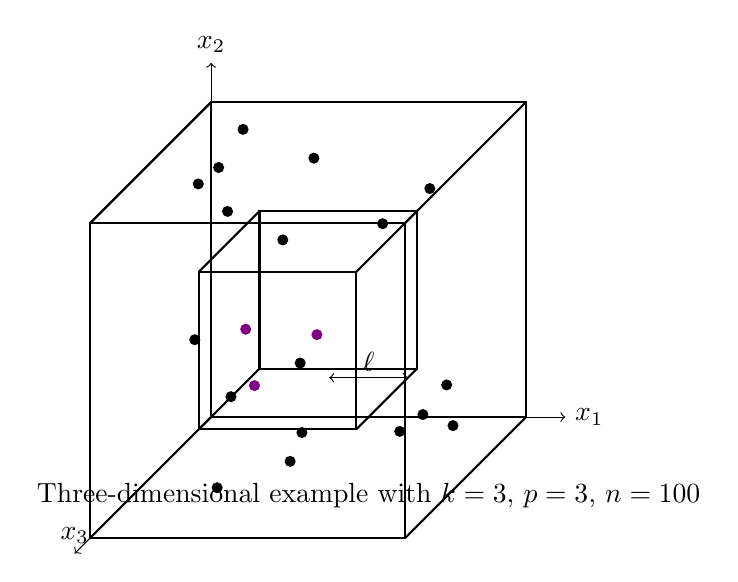
\begin{tikzpicture}
    % Draw the outer box
    \draw[thick] (0,0,0) -- (4,0,0) -- (4,4,0) -- (0,4,0) -- cycle;
    \draw[thick] (0,0,4) -- (4,0,4) -- (4,4,4) -- (0,4,4) -- cycle;
    \draw[thick] (0,0,0) -- (0,0,4);
    \draw[thick] (4,0,0) -- (4,0,4);
    \draw[thick] (4,4,0) -- (4,4,4);
    \draw[thick] (0,4,0) -- (0,4,4);

    % Add axis labels
    \draw[->] (0,0,0) -- (4.5,0,0) node[right] {$x_1$};
    \draw[->] (0,0,0) -- (0,4.5,0) node[above] {$x_2$};
    \draw[->] (0,0,0) -- (0,0,4.5) node[above] {$x_3$};

    % Draw the inner box
    \draw[thick] (1,1,1) -- (3,1,1) -- (3,3,1) -- (1,3,1) -- cycle;
    \draw[thick] (1,1,3) -- (3,1,3) -- (3,3,3) -- (1,3,3) -- cycle;
    \draw[thick] (1,1,1) -- (1,1,3);
    \draw[thick] (3,1,1) -- (3,1,3);
    \draw[thick] (3,3,1) -- (3,3,3);
    \draw[thick] (1,3,1) -- (1,3,3);

    % Generate 3 dots strictly inside the inner box
    \foreach \i in {1,...,3} {
        \pgfmathsetmacro{\x}{1 + rnd*2} % Random x between 1 and 3
        \pgfmathsetmacro{\y}{1 + rnd*2} % Random y between 1 and 3
        \pgfmathsetmacro{\z}{1 + rnd*2} % Random z between 1 and 3
        \fill[highlightcolor] (\x,\y,\z) circle (2pt);
    }

    % Generate random dots outside the inner box but within the outer box
    \foreach \i in {1,...,20} {
        \pgfmathsetmacro{\x}{rnd*4} % Random x between 0 and 4
        \pgfmathsetmacro{\y}{rnd*4} % Random y between 0 and 4
        \pgfmathsetmacro{\z}{rnd*4} % Random z between 0 and 4

        % Ensure the dot is strictly outside the inner cube
        \ifdim \x pt < 1 pt \fill[pointcolor] (\x,\y,\z) circle (2pt);
        \else \ifdim \x pt > 3 pt \fill[pointcolor] (\x,\y,\z) circle (2pt);
        \else \ifdim \y pt < 1 pt \fill[pointcolor] (\x,\y,\z) circle (2pt);
        \else \ifdim \y pt > 3 pt \fill[pointcolor] (\x,\y,\z) circle (2pt);
        \else \ifdim \z pt < 1 pt \fill[pointcolor] (\x,\y,\z) circle (2pt);
        \else \ifdim \z pt > 3 pt \fill[pointcolor] (\x,\y,\z) circle (2pt);
        \fi\fi\fi\fi\fi\fi
    }

    % Label the box length
    \draw[<->] (1.5,0.5,0) -- (2.5,0.5,0);
    \node at (2, 0.7, 0) {$\ell$};

    % Title
    \node[align=center] at (2,-1.0,0) {Three-dimensional example with $k=3$, $p=3$, $n=100$};
    \end{tikzpicture}
\end{center}

\subsection{Volume Analysis}
What are the volumes of the boxes in different dimensions?
\[
    \begin{aligned}
        \text{Outer Box Volumes:} \quad\\
        \text{For } p=1: \quad & V_{\text{big}} = 1 \\
        \text{For } p=2: \quad & V_{\text{big}} = 1 \\
        \text{For } p=3: \quad & V_{\text{big}} = 1 \\
        & \dots \\
        \text{For } p=p: \quad & V_{\text{big}} = 1 \\
        \end{aligned}
        \quad \quad
        \begin{aligned}
        \text{Inner Box Volumes:} \quad\\
        \text{For } p=1: \quad & V_{\text{small}} = \ell < 1 \\
        \text{For } p=2: \quad & V_{\text{small}} = \ell^2 \\
        \text{For } p=3: \quad & V_{\text{small}} = \ell^3 \\
        & \dots \\
        \text{For } p=p: \quad & V_{\text{small}} = \ell^p \\
    \end{aligned}
\]

\section{Distance Metrics Implementation}
\subsection{Code Examples in Julia}
The following code examples demonstrate how to calculate different distance metrics and explore the effects of dimensionality using Julia.

\begin{tcolorbox}[width=\textwidth, left=-6mm, sharp corners, boxrule=0pt, title=\textbf{Import required packages}]
  \begin{minted}[fontsize=\small]{julia}
    # Import the Distances package for various distance metrics
    using Distances

    # Import LinearAlgebra for norm calculations
    using LinearAlgebra 
  \end{minted}
\end{tcolorbox}

\begin{tcolorbox}[width=\textwidth, left=-6mm, sharp corners, boxrule=0pt, title=\textbf{Create two random 2D points}]
  \begin{minted}[fontsize=\small]{julia}
    # Generate a random 2D point
    x = rand(2) 

    # Output will be something like:
    # 2-element Vector{Float64}:
    #   0.11715724827332152
    #   0.8703834178825096

    # Generate another random 2D point
    y = rand(2)

    # Output will be something like:
    # 2-element Vector{Float64}:
    #   0.983074530416966
    #   0.9654697003440244
  \end{minted}
\end{tcolorbox}

\begin{tcolorbox}[width=\textwidth, left=-6mm, sharp corners, boxrule=0pt, title=\textbf{Calculate different distance metrics}]
  \begin{minted}[fontsize=\small]{julia}
    # Calculate Euclidean distance between x and y
    # This is the square root of the sum of squared differences
    euclidean_distance = Euclidean()(x,y)
    # Output: 0.8711223453840379

    # Calculate Minkowski distance with p=2 (equivalent to Euclidean)
    minkowski_distance = Minkowski(2)(x,y)
    # Output: 0.8711223453840379

    # Calculate Hamming distance (counts the number of differences)
    hamming_distance = Hamming()(x,y)
    # Output: 2 (both elements are different)

    # Alternative way to calculate Euclidean distance using norm
    norm_distance = norm(x-y)
    # Output: 0.8711223453840379
  \end{minted}
\end{tcolorbox}

\begin{tcolorbox}[width=\textwidth, left=-6mm, sharp corners, boxrule=0pt, title=\textbf{Implementing the box size formula}]
  \begin{minted}[fontsize=\small]{julia}
    # Define the function for calculating box side length
    # This implements our formula: ℓ = (k/n)^(1/p)
    L(p) = @. (k/n)^(1/p)

    # Define a range of dimensions to explore
    p = [1, 2, 3, 10, 20, 100]

    # Set number of total points and desired points inside box
    n = 1000  # Total number of points
    k = 11    # Desired number of points inside box

    # Calculate box side length for each dimension
    L.(p)

    # Output:
    # 6-element Vector{Float64}:
    #  0.011                 # For p=1
    #  0.10488088481701516   # For p=2
    #  0.22239800905693158   # For p=3
    #  0.6369997597182926    # For p=10
    #  0.7981226470400978    # For p=20
    #  0.9559032250692122    # For p=100

    # Notice how the box size approaches 1 as dimensions increase!
  \end{minted}
\end{tcolorbox}

\begin{tcolorbox}[width=\textwidth, left=-6mm, sharp corners, boxrule=0pt, title=\textbf{Experiment: Average distance in high dimensions}]
  \begin{minted}[fontsize=\small]{julia}
    # Experiment to show how average distance grows in higher dimensions
    N = 500      # Number of point pairs
    d = 5        # Number of dimensions
    D = 0.0      # Sum of distances (initialize to zero)

    # Generate N pairs of random points and calculate average distance
    for _ = 1:N
      x = rand(d)  # Random point in d-dimensional space
      y = rand(d)  # Another random point
      D += norm(x - y)  # Add Euclidean distance to total
    end

    # Print total sum of distances
    println(D)
    # Output: 450.01189208407664

    # Average distance would be D/N (approximately 0.90 for d=5)
    # This value grows as d increases!
  \end{minted}
\end{tcolorbox}

\begin{tcolorbox}[width=\textwidth, left=-6mm, sharp corners, boxrule=0pt, title=\textbf{ Experiment: Distance to nearest edge}]
  \begin{minted}[fontsize=\small]{julia}
    # This computes the minimum distance from random points to nearest edge
    # using infinity norm (maximum coordinate distance to edge)
    for _ = 1:100
      x = rand(d)  # Generate random point in d-dimensional unit hypercube

      # Calculate min distance to edge using infinity norm
      # For each coordinate, the distance to edge is min(xi, 1-xi)
      edge_distance = min(1-norm(x,Inf), norm(x,Inf))

      # As d increases, this distance tends to decrease!
    end
  \end{minted}
\end{tcolorbox}

\section{Distance Metrics in Detail}
\subsection{Properties of Distance}
When analyzing distances in spaces, we can encounter different behaviors:

\textbf{Divergence}: The distance between two points increases infinitely.

\textbf{Convergence}: The distance between two points converges to zero.

This is illustrated below:

\begin{center}
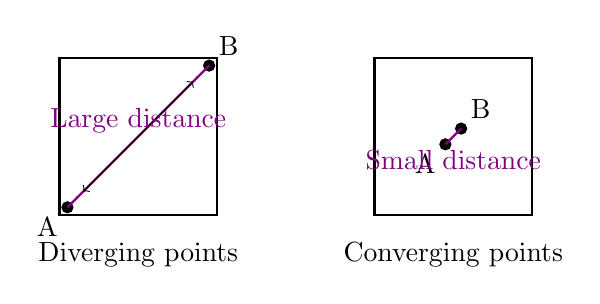
\begin{tikzpicture}
  % Draw the first box (divergence)
  \draw[thick] (1,1) rectangle (3,3);
  \node[align=center] at (2,0.5) {Diverging points};

  % Add points and distances
  \filldraw[black] (1.1,1.1) circle (2pt) node[below left] {A};
  \filldraw[black] (2.9,2.9) circle (2pt) node[above right] {B}; 
  \draw[thick, highlightcolor] (1.1,1.1) -- (2.9,2.9);
  \draw[<->] (1.3,1.3) -- (2.7,2.7);
  \node[highlightcolor] at (2,2.2) {Large distance};

  % Draw the second box (convergence)
  \draw[thick] (5,1) rectangle (7,3);
  \node[align=center] at (6,0.5) {Converging points};

  % Add points and lines for convergence
  \filldraw[black] (5.9,1.9) circle (2pt) node[below left] {A};
  \filldraw[black] (6.1,2.1) circle (2pt) node[above right] {B}; 
  \draw[thick, highlightcolor] (5.9,1.9) -- (6.1,2.1);
  \node[highlightcolor] at (6,1.7) {Small distance};

\end{tikzpicture}
\end{center}

\subsection{Important Properties of Distance Metrics}
Not all mathematical functions that measure ``difference" qualify as proper distance metrics. For example:

\textbf{Question}: Why is cosine distance not a true distance metric?

\textbf{Answer}: Cosine distance violates several properties required for a true metric:
\begin{outline}
    \1 It doesn't satisfy the triangle inequality
    \1 It doesn't satisfy the identity of indiscernibles (two different vectors can have a cosine distance of 0 if they point in the same direction but have different magnitudes)
\end{outline}

\section{K-Nearest Neighbors (KNN) Algorithm}
\subsection{Introduction to K-NN}

\textbf{Definition}: K-Nearest Neighbors (K-NN) is a non-parametric, instance-based learning algorithm used for both classification and regression.

\textbf{Core idea}: Objects are classified based on the majority class among their k nearest neighbors or prediction is made based on the average value of their k nearest neighbors.

\subsection{K-NN Algorithm Steps}
\begin{outline}[enumerate]
    \1 Choose a value for K (the number of neighbors)
    \1 Calculate the distance between the query point and all training points
    \1 Sort the distances and determine the K nearest neighbors
    \1 For classification: use majority voting among the K neighbors
    \1 For regression: use the average (or weighted average) of the K neighbors
\end{outline}

\subsection{Why K-NN Works}
K-NN is effective because:
\begin{outline}
    \1 It makes minimal assumptions about the underlying data distribution (non-parametric)
    \1 It can adapt to complex decision boundaries
    \1 It works well when data points from the same class form cohesive clusters
    \1 By considering multiple neighbors, it reduces sensitivity to noise
\end{outline}

In high-dimensional spaces, K-NN can still work effectively if the data points are not uniformly distributed, which helps mitigate the curse of dimensionality.

\subsection{K-NN Classification Example}
Consider the following scenario: Is the point marked with \textcolor{red}{?} positive or negative?

Parameters: $K = 3$ (we'll consider 3 nearest neighbors), $p = 2$ (2D space), $n = 16$ (16 total points)

\begin{center}
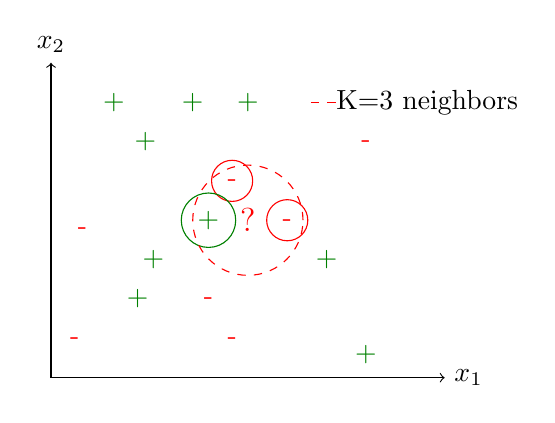
\begin{tikzpicture}
  % Draw axes
  \draw[->] (1,1) -- (6,1) node[right] {$x_1$};
  \draw[->] (1,1) -- (1,5) node[above] {$x_2$};

  % Plot positive and negative points
  \node[positiveclass] at (2.1, 2) {+};
  \node[positiveclass] at (5, 1.3) {+};
  \node[negativeclass] at (1.4, 2.9) {-};
  \node[negativeclass] at (5, 4) {-};
  \node[positiveclass] at (3.5, 4.5) {+};
  \node[positiveclass] at (2.3, 2.5) {+};
  \node[positiveclass] at (4.5, 2.5) {+};
  \node[negativeclass] at (3.3, 1.5) {-};
  \node[negativeclass, circle, draw] at (3.3, 3.5) {-};
  \node[positiveclass] at (2.2, 4) {+};
  \node[positiveclass] at (2.8, 4.5) {+};
  \node[positiveclass] at (1.8, 4.5) {+};
  \node[negativeclass] at (1.3, 1.5) {-};
  \node[positiveclass, circle, draw] at (3, 3) {+};
  \node[negativeclass, circle, draw] at (4, 3) {-};
  \node[negativeclass] at (3, 2) {-};

  % Plot the query point
  \node[specialpoint, font=\large] at (3.5, 3) {?};

  % Draw circles around the three nearest neighbors
  \draw[dashed, specialpoint] (3.5,3) circle (0.7);

  % Add legend
  \node[anchor=west] at (4.5,4.5) {K=3 neighbors};
  \draw[dashed, specialpoint] (4.3,4.5) -- (4.7,4.5);

\end{tikzpicture}
\end{center}

\textbf{Analysis}: The three nearest neighbors to the query point (?) are:
\begin{outline}
    \1 One positive point (+)
    \1 Two negative points (-)
\end{outline}

\textbf{Prediction}: Since the majority (2 out of 3) of the nearest neighbors are negative, we classify the query point as negative.

\subsection{Choosing K}
The choice of K is crucial in K-NN:
\begin{outline}
    \1 Smaller K values: More sensitive to noise, but can capture fine-grained patterns
    \1 Larger K values: More robust to noise, but may miss local patterns
    \1 For classification tasks, K should be odd to avoid ties
    \1 Common practice: Try different K values using cross-validation
\end{outline}

\subsection{Computational Complexity}
K-NN has the following computational requirements:
\begin{outine}[enumerate]
    \1 Calculation of distances between query point and all training points: $O(np)$ where $n$ is the number of training points and $p$ is the number of features
    \1 Sorting distances to find K nearest neighbors: $O(n \log n)$
    \1 Selecting K nearest neighbors: $O(K)$
\end{outline}

Overall complexity: $O(np + n \log n + K) \approx O(np + n \log n)$ since typically $K \ll n$.

\subsection{Handling Missing Data with K-NN}
Missing data is a common problem in real-world datasets. Consider a vector with missing values:
\[
    \begin{bmatrix}
        1 \\
        ? \\
        3 \\
        4 \\
        7 \\
        ? \\
        5
    \end{bmatrix}
\] 

There are several approaches to handling missing values:
\begin{outline}[enumerate]
    \1 Delete records with missing values (simple but loses information)
    \1 Replace with mean or median of the feature (fast but ignores correlations)
    \1 Use K-NN imputation:
            \2 Find K nearest neighbors based on non-missing features
            \2 Replace missing values with the average from these neighbors
            \2 This preserves relationships between features
\end{outline}

\textbf{Example}: If Maine is missing temperature data, taking the mean of all states would be biased by warm states like Texas and Arizona. Instead, K-NN would use temperatures from nearby northeastern states like New Hampshire and Vermont, providing a more accurate estimate.

\subsection{Formal K-NN Setup}
Mathematically, we can define the K-NN setup as:
\[
    \text{Data} = D = \{(x_i,y_i)\}^n_{i=1} \subset \mathbb{R}^p \times \{-1,1\}
\]
where:
\begin{outline}
    \1 $x_i \in \mathbb{R}^p$ are feature vectors
    \1 $y_i \in \{-1,1\}$ are binary class labels (can be extended to multi-class)
    \1 $n$ is the number of training examples
    \1 $p$ is the number of features
\end{outline}


\end{document}
